\documentclass[17pt]{beamer}
\usepackage{amssymb}
\usepackage{tikz}
\usetikzlibrary{arrows}
\useoutertheme{infolines}
\usetheme{default}
\author{Jeremy Ong}
\title{CRDTs in Production}
\begin{document}
\begin{frame}
  \titlepage
\end{frame}
\begin{frame}{Objective}
  \begin{itemize}
    \item Understand tradeoffs developers must consider when
      interfacing with an AP database (Riak specifically this talk) \pause
    \item Learn the knobs and levers at our disposal to manage
      consistency
  \end{itemize}
\end{frame}
\begin{frame}{Before you reject ACID...}
  ...understand the withdrawal symptoms
  \pause
  \begin{itemize}
  \item relationships between keys loosened
      \pause
  \item loss of immediate consistency
  \end{itemize}
  \pause
  Why leave in the first place?
\end{frame}
\begin{frame}{A not C please}
  Sometimes, availability is more valuable than \em immediate \em consistency.
  \pause
  \begin{itemize}
  \item Data sets are independent (user profile, shopping cart)
      \pause
  \item Writes or reads should still be allowable in the presence of
    network partition of hardware failure
      \pause
  \item Scalability is a real concern
  \end{itemize}
  \pause
  Desire: Cure the ACID hangover
\end{frame}
\begin{frame}{Low conflict intensity}
  Excellent candidates for a CRDT approach exhibit low conflict intensity:
  \pause
  \begin{itemize}
  \item One writer to a given key
    \pause
  \item Majority of writes come from a single writer
    \pause
  \item Writes occur sparingly
  \end{itemize}
\end{frame}
\begin{frame}{CRDT Preliminaries}
  Consensus: RDTs are replicated data types.

  \pause
  Does the C in CRDT mean:
  \begin{itemize}
    \item Convergent? or...
    \item Commutative?
  \end{itemize}
  \pause
  It depends!
  \begin{itemize}
    \item Convergent - state based RDTs
    \item Commutative - op based RDTs
  \end{itemize}
\end{frame}
\begin{frame}{CvRDTs}
  \begin{definition}
  Convergent RDT (CvRDT) - State based datatype that relies on
  merges to synchronize divergent replica copies (e.g. git)
  \end{definition}
  \pause
  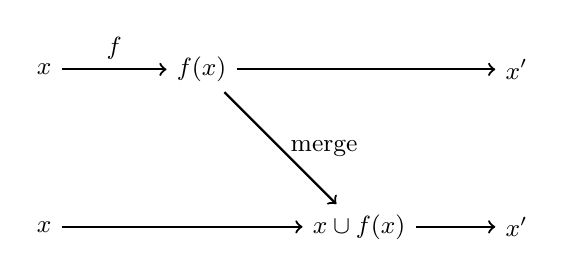
\begin{tikzpicture}[->,thick,font=\small,node distance=2cm]
    \node (1) {$x$};
    \node (2) [below of=1] {$x$};
    \node (3) [right of=1] {$f(x)$};
    \node (4) [right of=2] {};
    \node (5) [right of=4] {$x \cup f(x)$};
    \node (6) [right of=3] {};
    \node (7) [right of=5] {$x'$};
    \node (8) [right of=6] {$x'$};
    \path
    (1) edge node[above] {$f$} (3)
    (3) edge node[right] {merge} (5)
    (2) edge node {} (5)
    (3) edge node {} (8)
    (5) edge node {} (7)
    ;
  \end{tikzpicture}
\end{frame}
\begin{frame}{CmRDTs}
  \begin{definition}
    Commutative RDT (CmRDT) - Operation based datatype that replicates
    commutative operations across divergent replicas (e.g. Simon Says)
  \end{definition}
  \pause
  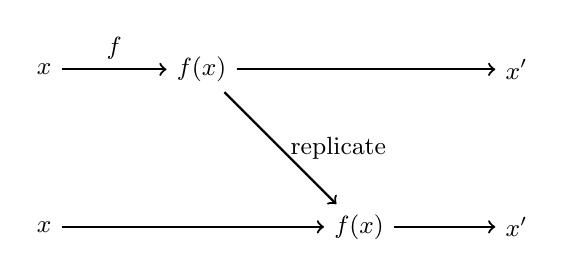
\begin{tikzpicture}[->,thick,font=\small,node distance=2cm]
    \node (1) {$x$};
    \node (2) [below of=1] {$x$};
    \node (3) [right of=1] {$f(x)$};
    \node (4) [right of=2] {};
    \node (5) [right of=4] {$f(x)$};
    \node (6) [right of=3] {};
    \node (7) [right of=5] {$x'$};
    \node (8) [right of=6] {$x'$};
    \path
    (1) edge node[above] {$f$} (3)
    (3) edge node[right] {replicate} (5)
    (2) edge node {} (5)
    (3) edge node {} (8)
    (5) edge node {} (7)
    ;
  \end{tikzpicture}
\end{frame}
\begin{frame}{CRDT Constraints}
  \begin{enumerate}
    \item Termination: At-source and/or downstream phases terminate
      when preconditions are satisfied.
      \pause
    \item Eventual Effect (violated by LWW):
      \[ \forall x_i \exists x_j \geq x_i \ni x_j \leq x_k \Leftrightarrow C\left(x_i\right) \subseteq C\left(x_k\right) \]
    \item \pause Convergence:
      \[ C\left(x_i\right) = C\left(x_j\right) \Rightarrow x_i \equiv x_j \]
  \end{enumerate}
\end{frame}
\begin{frame}{Application side CvRDT case study}
  CRDTs are an app developers responsibility (not just a database
  implementer's responsibility). Why?
  \pause

  Data denormalization!
  \pause
  Your database can't be expected to understand your schema.
  \pause

  Replica copies don't just exist in the database (think caching for example).
\end{frame}
\begin{frame}{Application side CvRDT case study}
  Merges vs Commutative ops (why not a CmRDT)
  \pause

  \begin{itemize}
    \item Maintainability - Avoid the merge function of doom (unless
      your data is canonical and merge-oriented)
      \pause
    \item Tight coupling of operation with resolution behavior
      \pause
    \item Resilience against schema changes
  \end{itemize}
\end{frame}
\begin{frame}{Shopping Cart Implementation}
  The schema is of the form $(d, f)$, a tuple combining shopping cart
  data ($d$) and the optional last operation used (initially $\varnothing$).
  \pause
  \begin{definition}
    \texttt{apply(d, f)} - Given data and an operation, returns the
    tuple $(f(d), f)$. Then write to the database.
  \end{definition}
\end{frame}
\begin{frame}{Shopping Cart Impl. 2}
  \begin{definition}
    \texttt{resolve$\left(\{s_1, s_2, \dots, s_n\}\right)$} - Given a
    list of siblings, returns the tuple $(f_2\circ f_3 \circ\cdots\circ f_n(d_1), \varnothing)$.
    Then issues a write to the database.
  \end{definition}
\end{frame}
\begin{frame}[fragile]{Example: AddToCart}
  \small
\begin{verbatim}
void AddToCart(Cart &cart,
               const Item &item,
               const unsigned int quantity) {
    if (cart.HasItem(item)) {
        cart.Get(item) += quantity;
    } else {
        cart.AddItem(item, quantity);
    }
}
\end{verbatim}
\end{frame}
\begin{frame}[fragile]{When things don't commute}
  The function \texttt{AddToCart} behaves nicely because it
  commutes. What about something like \texttt{RemoveFromCart}?
  \pause
  \small
\begin{verbatim}
void RemoveFromCart(Cart &cart,
                    const Item &item) {
    if (cart.HasItem(item)) {
        ... item removal code
    } else {
        // What should I do here?
\end{verbatim}
\pause
\begin{verbatim}
        // nothing
    }
}
\end{verbatim}
\end{frame}
\begin{frame}{Isn't that the same as LWW?}
  \pause
  No. \pause

  LWW would handle the case of duplicate removals of the same object,
  but doesn't handle conflicts of heterogeneous operations.
\end{frame}
\begin{frame}{Shopping Cart Summary}
The shopping cart is easy because
\begin{itemize}
  \item The cart behaves like a set of PN-counters
    \pause
  \item Operations that don't commute on a cart can simply be
    nullified if a condition is void
    \pause
\end{itemize}
We are essentially using \em deferred transactions\em.
\pause

Consider the behavior of the shopping cart if we did not use this
interface.
\end{frame}
\begin{frame}{Relaxed CRDT constraints}
  \begin{enumerate}
    \item Termination: unchanged
      \pause
    \item Eventual Effect (relaxed): For every operation on some
      $x_i$, an attempt to perform that operation is eventually
      performed on all later replica copies.
    \item \pause Convergence (relaxed): Replicas converge in the
      absence of write conflict but the worst case effects of a
      conflict are loss of operation.
  \end{enumerate}
\end{frame}
\begin{frame}{Differences from a standard transaction}
  \begin{itemize}
    \item Op cancellation is code dependent \pause
    \item Client is not immediately aware of issue (it's eventual) \pause
    \item Local to a single object. \pause
    \item Passive vs active merge resolution
  \end{itemize}
\end{frame}
\begin{frame}{Improving our database interface}
  \begin{itemize}
    \item Spawn events when an op gets canceled so client can be
      notified \pause
    \item Have our update function take a precondition function as an
      additional argument instead of embedding it in the code \pause
    \item Handling multiple key updates... ignore for now
  \end{itemize}
\end{frame}
\begin{frame}{Interface Flow}
  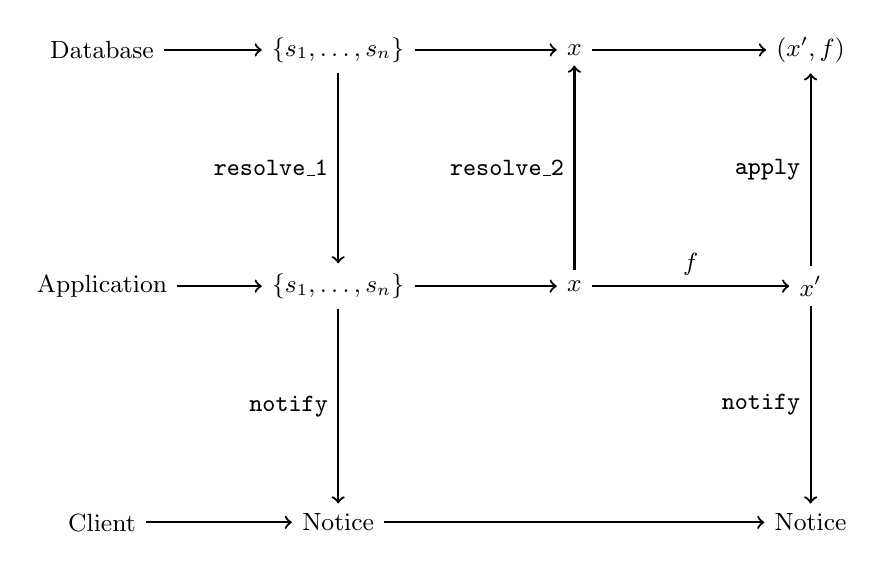
\begin{tikzpicture}[->, thick, font=\small, node distance=3cm]
    \node (client) {Client};
    \node (client1) [right of=client] {Notice};
    \node (client2) [right of=client1] {};
    \node (client3) [right of=client2] {Notice};
    \node (app) [above of=client] {Application};
    \node (app1) [right of=app] {$\{s_1, \dots, s_n\}$};
    \node (app2) [right of=app1] {$x$};
    \node (db) [above of=app] {Database};
    \node (db1) [right of=db] {$\{s_1, \dots, s_n\}$};
    \node (db2) [right of=db1] {$x$};
    \node (app3) [right of=app2] {$x'$};
    \node (db3) [right of=db2] {$(x', f)$};
    \path
    (app) edge node {} (app1)
    (db) edge node {} (db1)
    (client) edge node {} (client1)
    (client1) edge node {} (client3)
    (db2) edge node {} (db3)
    (db1) edge node[left] {\texttt{resolve\_1}} (app1)
    (app1) edge node[left] {\texttt{notify}} (client1)
    (app1) edge node {} (app2)
    (app2) edge node[above] {$f$} (app3)
    (db1) edge node {} (db2)
    (app2) edge node[left] {\texttt{resolve\_2}} (db2)
    (app3) edge node[left] {\texttt{apply}} (db3)
    (app3) edge node[left] {\texttt{notify}} (client3)
    ;
  \end{tikzpicture}
\end{frame}
\begin{frame}{Read/Write Quorums}
  How do we choose what R or W should be? \pause

  There are three different database interactions to consider:

  \begin{enumerate}
    \item \texttt{resolve\_1}: initial read which may return multiple
      siblings \pause
    \item \texttt{resolve\_2}: write for resolving conflicts \pause
    \item \texttt{apply}: write to record a new operation
  \end{enumerate}
\end{frame}
\begin{frame}{\texttt{resolve\_1} and \texttt{apply}}
  \texttt{resolve\_1} is application dependent \pause

  Use of a high R value will:
  \begin{itemize}
  \item (-) reduce availability \pause
  \item (+) keep sibling count low \pause
  \item (+) improve consistency \pause
  \end{itemize}

  \texttt{apply} is the opposite of \texttt{resolve\_1} and has similar characteristics
\end{frame}
\begin{frame}{\texttt{resolve\_2}}
  When attempting to flatten siblings, additional care must be taken. \pause
  \begin{itemize}
    \item What if multiple writers attempt to flatten a list of
      siblings at the same time? \pause
    \item What if a netsplit occurs? \pause
  \end{itemize}

  W should be at least $\lceil Q\slash 2 \rceil$ to prevent conflicts
  during a netsplit
\end{frame}
\begin{frame}{Handling a \texttt{resolve\_2} conflict}
  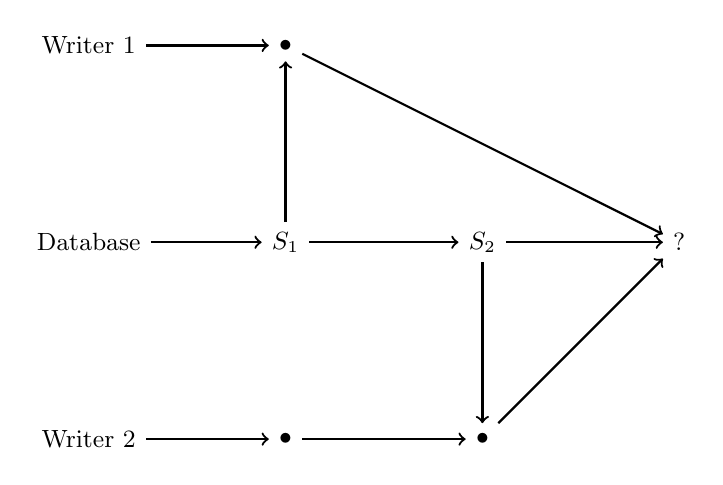
\begin{tikzpicture}[->, thick, font=\small, node distance=2.5cm]
    \node (w1) {Writer 1};
    \node (db) [below of=w1] {Database};
    \node (w2) [below of=db] {Writer 2};
    \node (w11) [right of=w1] {$\bullet$};
    \node (w21) [right of=w2] {$\bullet$};
    \node (w22) [right of=w21] {$\bullet$};
    \node (db1) [right of=db] {$S_1$};
    \node (db2) [right of=db1] {$S_2$};
    \node (db3) [right of=db2] {?};
    \path
    (w1) edge node {} (w11)
    (w2) edge node {} (w21)
    (w21) edge node {} (w22)
    (db) edge node {} (db1)
    (db1) edge node {} (w11)
    (db2) edge node {} (w22)
    (w22) edge node {} (db3)
    (w11) edge node {} (db3)
    (db1) edge node {} (db2)
    (db2) edge node {} (db3)
    ;
  \end{tikzpicture}
\end{frame}
\begin{frame}{When writes collide}
  If multiple writers flatten siblings and save it to the database,
  there are a few options \pause
  \begin{itemize}
    \item Arbitrarily ignore all of them but one \pause
    \item Enforce that flattening can only occur from one writer \pause
  \end{itemize}

  The tradeoff, as always, is availability over consistency.
\end{frame}
\begin{frame}{What about when\dots}
  \dots the result of a flatten operation conflicts with a normal apply?
  \pause

  Assuming all writers are well-behaved and read first with the
  \texttt{resolve} interface, it's safe to ignore the result of the
  flatten operation.
\end{frame}
\begin{frame}{Another kind of conflict}
  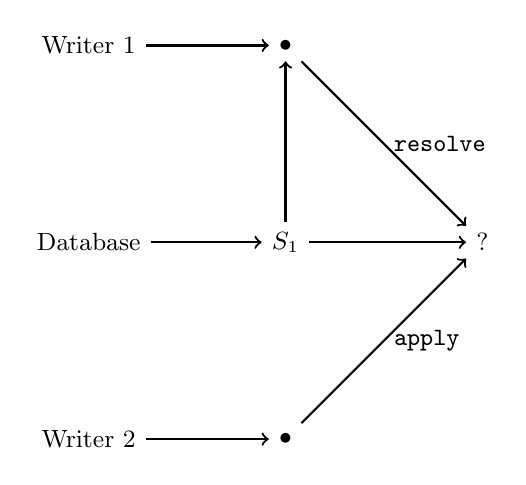
\begin{tikzpicture}[->, thick, font=\small, node distance=2.5cm]
    \node (w1) {Writer 1};
    \node (db) [below of=w1] {Database};
    \node (w2) [below of=db] {Writer 2};
    \node (w11) [right of=w1] {$\bullet$};
    \node (w21) [right of=w2] {$\bullet$};
    \node (db1) [right of=db] {$S_1$};
    \node (db2) [right of=db1] {?};
    \path
    (w1) edge node {} (w11)
    (w2) edge node {} (w21)
    (db) edge node {} (db1)
    (db1) edge node {} (w11)
    (w21) edge node[right] {\texttt{apply}} (db2)
    (w11) edge node[right] {\texttt{resolve}} (db2)
    (db1) edge node {} (db2)
    ;
  \end{tikzpicture}
\end{frame}
\begin{frame}{Handling all conflicts}
  Many strategies exist for merging siblings. Important takeaways:
  \pause
  \begin{itemize}
    \item Make sure you can handle all cases, or some sets of siblings
      will be stuck (your \texttt{resolve} function should not have an
      exit path that doesn't result in a valid write). \pause
    \item The best strategy isn't always the most complicated. With
      low conflict intensity, the majority of cases will be simple
  \end{itemize}
\end{frame}
\begin{frame}{Writer hierarchy}
  One option suitable for some applications is a writer hierarchy.
  \pause

  Given a list of siblings $\{s_1, \dots, s_n\}$, first sort them in
  order by the priority of their sources before composing the embedded
  functions. \pause

  e.g. In an implementation of an email browser client, we may want to
  prioritize one tab over another.
\end{frame}
\begin{frame}{Note about multi-key transactions}
  This is hard, but you can\dots \pause

  \dots Changed my mind, this is very hard. Just denormalize more or
  use indices \pause

  If you absolutely must impose a strict transactional relationship
  between two keys, there is a scheme to ensure that if an op on one
  key of the transaction fails, the op should fail on the other side
  (through the usage of inverse operators). Outside the scope.
\end{frame}
\begin{frame}{Possible shifts to existing database usage}
  \begin{itemize}
    \item Tighter integration between application code and database
      code (active app specific conflict resolution) \pause
    \item Pub/sub api to allow an application to listen for changes to
      a given key \pause
    \item Fully featured db client API to allowing setting op,
      precondition, and other metadata \pause
  \end{itemize}
\end{frame}
\begin{frame}{Conclusion}
  \begin{itemize}
    \item If you can reduce conflict intensity in other areas of the
      system, do it.
    \item This approach will not provide guaranteed consistency like a
      canonical CRDT, but is better than LWW.
    \item Consistency is a spectrum and the developer can lean in
      either direction. You must choose!
  \end{itemize}
\end{frame}
\end{document}
